\documentclass{prova}

\usepackage{amssymb}

\renewcommand{\sin}{\mbox{sen}\,}
\newcommand{\ds}{\displaystyle}

\professor{Prof.\@ Adriano Barbosa}
\disciplina{C\'alculo Diferencial e Integral II}
\avaliacao{Final}
\curso{Eng. de Energia}
\data{14/12/2018}

\begin{document}
	\cabecalho{5}  % o numero 5 indica a qnt de quadros na tabela de nota

	\textbf{Todas as respostas devem ser justificadas.}
	\begin{questionario}
        \q{Resolva a integral definida $\ds\int_1^{e} \frac{\sin{(\ln
        x)}}{x}\ dx$.}
        \q{Calcule a integral indefinida $\ds\int e^x x^2\ dx$.}
        \q{Resolva a equa\c{c}\~ao diferencial $2ye^{y^2}y' = 2x+3\sqrt{x}$.}
        \q{Calcule a s\'erie de Taylor da fun\c{c}\~ao $f(x)=\sin{x}$ centrada em
        $a=\pi/2$ e determine seu raio de converg\^encia.}
        \q{Tri\^angulos ret\^angulos s\~ao construidos como na figura abaixo. Cada
        tri\^angulo tem altura 1 e sua base tem medida igual a hipotenusa do
        tri\^angulo anterior. Determine se a s\'erie $\ds\sum_{n=1}^\infty h_n$,
        formada pela soma das hipotenusas desses tri\^angulos, \'e convergente ou
        divergente.}
        \begin{figure}[h]
            \centering
            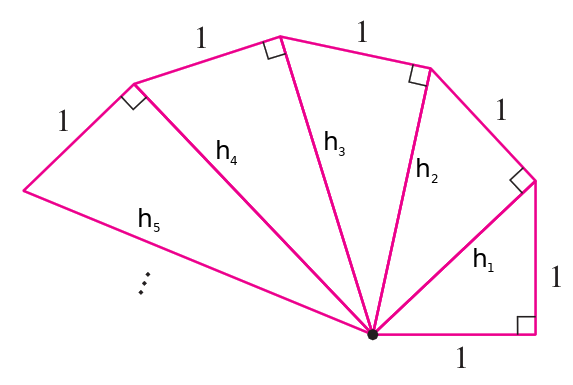
\includegraphics[width=0.5\textwidth]{triangulos.png}
        \end{figure}
	\end{questionario}
\end{document}
